%%%%%%%%%%%%%%%%%%%%%%%%%%%%%%%%%%%%%%%%%
% Simple Sectioned Essay Template
% LaTeX Template
%
% This template has been downloaded from:
% http://www.latextemplates.com
%
% Note:
% The \lipsum[#] commands throughout this template generate dummy text
% to fill the template out. These commands should all be removed when 
% writing essay content.
%
%%%%%%%%%%%%%%%%%%%%%%%%%%%%%%%%%%%%%%%%%

%----------------------------------------------------------------------------------------
%	PACKAGES AND OTHER DOCUMENT CONFIGURATIONS
%----------------------------------------------------------------------------------------

\documentclass[11pt]{article} % Default font size is 12pt, it can be changed here

\usepackage[T1]{fontenc}
\usepackage[polish]{babel}
\usepackage[utf8]{inputenc}
\usepackage{lmodern}
\selectlanguage{polish}

\usepackage{geometry} % Required to change the page size to A4
\geometry{a4paper} % Set the page size to be A4 as opposed to the default US Letter

\usepackage{graphicx} % Required for including pictures

\usepackage{float} % Allows putting an [H] in \begin{figure} to specify the exact location of the figure
\usepackage{wrapfig} % Allows in-line images such as the example fish picture

\usepackage{lipsum} % Used for inserting dummy 'Lorem ipsum' text into the template

\linespread{1.2} % Line spacing

%\setlength\parindent{0pt} % Uncomment to remove all indentation from paragraphs


\graphicspath{{Pictures/}} % Specifies the directory where pictures are stored

\begin{document}

%----------------------------------------------------------------------------------------
%	TITLE PAGE
%----------------------------------------------------------------------------------------

\begin{titlepage}

\newcommand{\HRule}{\rule{\linewidth}{0.5mm}} % Defines a new command for the horizontal lines, change thickness here

\center % Center everything on the page

\textsc{\LARGE Politechnika Poznańska}\\[0.5cm] % Name of your university/college
\textsc{\large Wydział Maszyn Roboczych i Transportu}\\[2.5cm] % Major heading such as course name

\textsc{\LARGE mgr inż. Natalia Lewandowska}\\[2.5cm] % Minor heading such as course title

\textsc{\large Metodologia i zasada redagowania prac naukowych}\\[0.1cm] 
\textsc{\small roboczy temat pracy:}\\[0.1cm] 

\HRule \\[0.5cm]
{ \huge \bfseries CFD analysis of blood flow through the arteries for diagnostic purposes}\\[0.4cm] % Title of your document
\HRule \\[0.5cm]

%\begin{minipage}{0.4\textwidth}
\begin{flushleft} \large
\emph{opiekun naukowy:}\\
prof. dr hab. inż. Michał \textsc{Ciałkowski}\\[6cm] % Your name
\end{flushleft}
%\end{minipage}
%~
%\begin{minipage}{0.4\textwidth}
%\begin{flushright} \large
%\emph{} \\
%\textsc{} % Supervisor's Name
%\end{flushright}
%\end{minipage}\\[4cm]

{\large \today}\\[0.5cm] % Date, change the \today to a set date if you want to be precise

%\includegraphics{Logo}\\[1cm] % Include a department/university logo - this will require the graphicx package

\vfill % Fill the rest of the page with whitespace

\end{titlepage}

%----------------------------------------------------------------------------------------
%	TABLE OF CONTENTS
%----------------------------------------------------------------------------------------

\tableofcontents % Include a table of contents

\newpage % Begins the essay on a new page instead of on the same page as the table of contents 

%----------------------------------------------------------------------------------------
%	OBSZAR I KIERUNEK BADAŃ
%----------------------------------------------------------------------------------------

\section{Obszar i kierunek badań} % Major section

\underline{Ogólny obszar badań}:  mechanika płynów, komputerowa mechanika płynów (CFD).\\
\\
\underline{Podobszar badań} (specjalistycznie zagadnienia): 

\begin{itemize} 
\item przepływ nieściśliwy cieczy nienewtonowskich, 
\item przepływy z kanałach o ściankach elastycznych,
\item zagadnienia z dziedziny chirurgii naczyniowej i neurochirurgii w kontekście geometrii tętnic i biomechaniki przepływu. \\
\end{itemize}


%----------------------------------------------------------------------------------------
%	LITERATURA
%----------------------------------------------------------------------------------------

\section{Literatura wymagana do realizacji celu rozprawy doktorskiej} % Major section

%------------------------------------------------

\subsection{Gdzie szukano literatury} % Sub-section

Głównym źródłem poszukiwanej literatury są czasopism związanych z biomechaniką przepływów i chirurgią naczyniową. Najważniejsze z nich to: 
\begin{itemize} 
\item Journal of Biomechanics (lista ministerialna: 30 pkt.)
\item Journal of Biomechanical Engineering (25 pkt.)
\item Stroke (45 pkt.)
\item Journal of Vascular Surgery (35 pkt.)
\item Journal of Surgical Research (30 pkt.)
\item European Journal of Vascular and Endovascular Surgery (35 pkt.) 
\end{itemize}
Prace dot. właściwości ścianek tętnic, modelu krwi i wzrostu tętniaków są poszukiwane głównie w takich czasopismach jak np.:
\begin{itemize} 
\item Proceedia Engineering, 
\item Computer Methods in Biomechanics and Biomedical Engineering (25 pkt.) 
\item International Journal for Numerical Methods in Biomedical (30 pkt.)
\item Journal of the Mechanical Behaviour of Biomedical Materials (35 pkt.) 
\end{itemize}

%------------------------------------------------

\subsection{Literatura ogólna} % Sub-sub-section

Literatura ogólna dotyczy głównie mechaniki płynów. Poznanie podstawowych zjawisk przepływowych i ich matematycznego opisu jest kluczowe dla zrozumienia procesów przepływowych w tętnicy. Główne źródła wykorzystywane do nauki to:

\begin{enumerate} 
\item Prosnak W., Mechanika Płynów tom I, PWN, Warszawa 1970
\item Ciałkowski M., Mechanika Płynów, Wydawnictwo Politechniki Poznańskiej, Poznań 2015
\item White F., Fluid Mechanics 8th edition, McGraw-Hill, 2011 
\item von Karman T., Mechanical Similitude and Turbulence, Washington 1931
\item Elsner J., Turbulencja Przepływów, PWN, Warszawa 1987
\end{enumerate}

Do literatury ogólnej zakwalifikowano również literaturę z dziedziny numeryki, silnie korelującą z mechaniką płynów. Ponadto uzupełniania jest wiedza z matematyki, więc literatura ogólna obejmuje również podręczniki z matematyki:
\begin{enumerate}
\item Bjorck A., Dahlquist G., Metody numeryczne, PWN, 1987
\item Kincaid D., Cheney W., Analiza numeryczna, WNT, 2007
\item Maćkiewicz A., Algorytmy algebry liniowej, Wydawnictwo Politechniki Poznańskiej, 2002
\end{enumerate}

%------------------------------------------------

\subsection{Literatura specjalistyczna} % Sub-sub-section

Literatura specjalistyczna obejmuje głównie zagadnienia związane z biomechaniką przepływów. Są to głównie artykuły opisujące zachowanie się różnych parametrów przepływowych krwi pod wpływem modyfikacji geometrii. Istotą literatury specjalistycznej jest  wyjaśnienie zjawisk przepływowych. Wiele artykułów, które kwalifikują się do literatury specjalistycznej dotyczą teoretycznego opisu zjawisk np. pompowania krwi przez serce, zachowania się ciśnienia i prędkości krwi po jej „wypchnięciu” z komorę sercowej oraz tłumaczą one proces formowania się tętniaków. Przykłady artykułów: 

\begin{enumerate}
\item Catanho, M., Sinha, M., Vijayan, V. BENG 221-Mathematical Methods in Bioengineering Model of Aortic Blood Flow Using the Windkessel Effect. (2012).
\item Morales, H. G., Larrabide, I., Geers, A. J., Aguilar, M. L., Frangi, A. F., Newtonian and non-Newtonian blood flow in coiled cerebral aneurysms, J. Biomech. 46, 2158–2164, 2013.
\item Golam Rabby, M., Razzak, A., Mamun Molla, M., Pulsatile non-Newtonian blood flow through a model of arterial stenosis. Procedia Eng. 56, 225–231, 2013.
\item Reichmann, B. L., Flow Velocities in the External Carotid Artery Following Carotid Revascularization, European Journal of Vascular and Endovascular Surgery, doi:10.1016/j.ejvs.2013.07.002, 2013
\item Wesseling, K. H., Jansen, J. R. C., Settels, J. J., Schreuder, J. J., Computation of aortic flow from pressure in humans using a nonlinear, three-element model., Journal of Applied Physiology, doi: 10.1152/jappl.1993.74.5.2566, 2018
\item Bijari, P. B., Wasserman, B. A., Steinman, D. A., Carotid bifurcation geometry is an independent predictor of early wall thickening at the carotid bulb, Stroke, doi:10.1161/STROKEAHA.113.003454, 2014
\end{enumerate}

%------------------------------------------------

\subsection{Literatura wysokospecjalistyczna} % Sub-sub-section

Literatura wysokospecjalistyczna dotyczy głównie zastosowań metod numerycznych w przepływie krwi przez tętnice. Obejmuje ona artykuły naukowe, materiały konferencyjne i rozprawy doktorskie. Zagadnienia występujące w literaturze wysokospecjalistycznej dotyczą głównie symulacji przepływu przez tętnicę szyjną i fragmentów koła Willisa (zbioru rozgałęzionych tętnic mózgowych). Rozważane są również przypadki, w których autor nie precyzuje rodzaju tętnicy, natomiast skupia się bardziej na parametrach przepływowych i ich wpływie na niektóre schorzenia naczyniowe. 
\begin{enumerate}
\item Olufsen, M. S., Numerical Simulation and Experimental Validation of Blood Flow in Arteries with Structured-Tree Outflow Conditions., Ann. Biomed. Eng. 28, 1281–1299, 2000
\item Van Steenhoven, A. A., Van De Vossea G., Experimental and Numerical Analysis of Carotid Arterv Blood Flow, Monogr Atheroscler. Basel, Karger 15, 250–260, 1990
\item Sarkar Shishir, S., Abdul Karim Miah M., Sadrul Islam A.,Toufique Hasan A., Blood Flow Dynamics in Cerebral Aneurysm - A CFD Simulation. Procedia Eng. 105, 919–927, 2015.
\item Shamloo, A., Nejad M. A., Saeedi M., Fluid–structure interaction simulation of a cerebral aneurysm: Effects of endovascular coiling treatment and aneurysm wall thickening, J. Mech. Behav. Biomed. Mater. 74, 72–83, 2017
\end{enumerate}

%------------------------------------------------

\subsection{Literatura pomocnicza - metodyczna} % Sub-sub-section

Literatura typu metodycznego wspierająca wyciągniecie właściwych wniosków ze zrealizowanych badań oraz prawidłowe napisanie rozprawy doktorskiej:
\begin{enumerate}
\item Wisłocki K., Metodologia i redakcja prac naukowych, Wydawnictwo Politechniki Poznańskiej, 2013
\end{enumerate}


Do literatury pomocniczej zakwalifikowano również wszelkiego rodzaju tutoriale, podręczniki użytkownika i materiały pomocnicze do wykorzystywanego oprogramowania:
\begin{itemize}
\item do tworzenia geometrii i siatek: Ansys ICEM CFD,
\item do analizy numerycznej: Ansys Fluent oraz OpenFOAM,
\item podręczniki do nauki programowania w języku Python i C++.
\end{itemize}



%------------------------------------------------

\subsection{Literatura - inna} % Sub-sub-section

W rozprawie doktorskiej będą przedstawione rozszerzenone wyniki badań, które rozpoczęto już przy pisaniu pracy magisterskiej. Część z nich już opublikowano w ramach materiałów konferencyjnych. Będą one bazą do napisania pracy doktorskiej. Poniższe artykuły zostaną również opublikowane (w rozszerzonej wersji) w monografii \textbf{\textit{“New Developments on Computational Methods and Visualization in Biomechanics and Biomedical Engineering”}} wydawanej przed wydawnictwo Springer.
\begin{enumerate}
\item Ciałkowski, M., Lewandowska N., Micker M., The Impact of Patches on Blood Flow Disorders in Carotid Artery, 15th International Symposium on Computer Methods in Biomechanics and Biomedical Engineering, 2018
\item Lewandowska, N., Ciałkowski M., Micker M.: Numerical Study of Carotid Bifurcation Angle Effect on Blood Flow Disorders, 15th International Symposium on Computer Methods in Biomechanics and Biomedical Engineering, 2018
\item Micker, M., Lewandowska N., Ciałkowski M., Physical Foundations for the Selection of Diagnostic Parameters of Atherosclerotic Plaque Growth, 15th International Symposium on Computer Methods in Biomechanics and Biomedical Engineering, 2018
\end{enumerate}



%----------------------------------------------------------------------------------------
%	ZAKRES WIEDZY I NIEWIEDZY
%----------------------------------------------------------------------------------------

\section{Zakres wiedzy i niewiedzy} % Major section

%------------------------------------------------

\subsection{Zakres wiedzy} % Sub-section

Stan wiedzy dotyczący biomechaniki przepływów jest bardzo wysoko rozwinięty:
\begin{itemize}
\item istnieją modele odwzorowujące bardzo dobrze właściwości reologiczne krwi, które zaimplementowane do modelu tętnicy dają bardzo dobre rezultaty;
\item bardzo solidne podstawy analityczne opisujące przepływ płynu nienewtonowskiego za pomocą równania zachowania pędu;
\item duża baza badań reologicznych krwi, właściwości wytrzymałościowych ścianek tętnicy;
\item bardzo dobrze udokumentowane zdjęcia tętniaków i zwężonych tętnic.
\end{itemize}



\subsection{Zakres niewiedzy} % Sub-sub-section

Pomysł na pracę zrodził się podczas współpracy z chirurgami naczyniowymi. Okazuje się, że nieznane są przyczyny występowania niektórych schorzeń. Przeprowadzane obecnie analizy zwykle odzwierciedlają obecny stan rzeczy, i bardzo rzadko na podstawie pola przepływowego dokonuje się przewidywań dalszego rozwoju zmiany chorobowej. Inaczej mówiąc, modele numeryczne przepływu krwi w tętnicach nie służą jako narzędzia diagnostyczne. Wykonywany w pracy doktorskiej model jest na bieżąco konsultowany z chirurgami, głównie ze względu na to, że będą oni w przyszłości wykorzystywać go do diagnostyki pacjentów.


Luki w wiedzy, których próba zapełnienia zostanie podjęta podczas realizacji przewodu doktorskiego:
\begin{itemize}
\item brak fizycznych podstaw kwalifikacji pacjentów do operacji usunięcia złogów (chirurdzy zwykle kwalifikują pacjentów na podstawie przeczucia i doświadczenia),
\item brak znormalizowanych geometrii łatek operacyjnych wszywanych w miejsce rozcięcia tętnicy,
\item do dzisiaj nie wiadomo, dlaczego niektóre tętniaki pękają a inne przez lata nie zmieniają swoich wymiarów. 
\end{itemize}

%----------------------------------------------------------------------------------------
%	PROBLEM BADAWCZY
%----------------------------------------------------------------------------------------

\section{Problem badawczy}

Najważniejszym problemem badawczym jest umożliwienie stosowania modelu jako narzędzie diagnostyczne. Rozwiązanie tego problemu wymaga wdrożenia wielu parametrów, które będą traktowane jako dane wejściowe o zmiennych wartościach. Model musi być również obudowany w przyjazny chirurgom interfejs.

%----------------------------------------------------------------------------------------
%	ZASADNICZY CEL PRACT
%----------------------------------------------------------------------------------------

\section{Zasadniczy cel pracy}

Model numeryczny jako narzędzie diagnostyczne.\\

Cele pośrednie:
\begin{itemize}
\item na podstawie analizy pola przepływowego, głównie prędkości i wielkości tworzących się wirów, być w stanie określić prędkość narastania złogów w tętnicy             i na tej podstawie określić po jakim czasie poziom zablokowania światła tętnicy jest na tyle duży, że ryzyko operacyjne związane z usunięciem złogów jest mniejsze od ryzyka „zatkania” tętnicy,
\item FSI (połączenie analizy pola przepływowego z analizą wytrzymałościową materiałów) tętniaków: stworzenie symulacji pozwalającej przewidzieć proces narastania tętniaka i czas jego pęknięcia.
\end{itemize}


%----------------------------------------------------------------------------------------
%	HARMONOGRAM PRAC
%----------------------------------------------------------------------------------------

\section{Harmonogram prac}

Na rysunku 1 przedstawiono harmonogram prac. Koncepcje prowadzenia badań szczegółowo opisano w rozdziale 7. 

\begin{figure}[H] 
\center{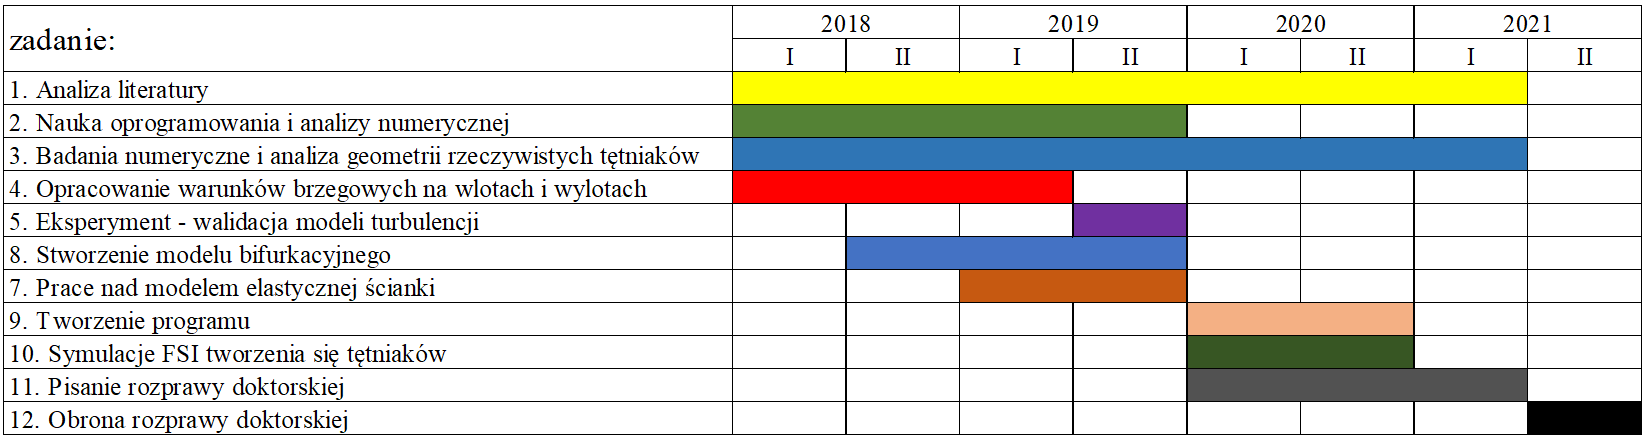
\includegraphics[width=1\linewidth]{harmonogram}}
\caption{Harmonogram prac}
\label{fig:speciation}
\end{figure}

%----------------------------------------------------------------------------------------
%	KONCEPCJA BADAŃ
%----------------------------------------------------------------------------------------

\section{Koncepcja badań}

Analiza literatury trwa przez cały okres studiów doktoranckich. Pierwsze dwa lata doktoratu obejmują naukę oprogramowania i języków programowania: zapoznanie się z oprogramowaniem do FSI, naukę języków: C++ i Python pod kątem analizy danych i tworzenia interfejsu. Nauka oprogramowania uwzględnia również zdobycie doświadczenia poprzez modelowanie w opensource’wym programie OpenFOAM. 


Zadania postawione na pierwszy rok doktoratu są już w większości zrealizowane. Opracowano autorski program do tworzenia funkcji pulsacyjnego profilu prędkości na podstawie zdjęć z ultrasonografu. Program po wczytaniu obrazu, wyznacza funkcję prędkości poprzez aproksymację wielomianem metodą najmniejszych kwadratów (Rys.2). Następnie funkcja prędkości jest wykorzystywana do wyznaczenia profilu ciśnienia na wylocie z tętnicy przy wykorzystaniu modelu Windkessela. Oprócz profilu prędkości, danymi wejściowymi do modelu Windkessela są również parametry związane z lepkością, gęstością krwi oraz geometrią tętnicy. Program jest napisany w języku Python i kod dostępny jest na Githubie. Kolejne pół roku zostanie przeznaczone na dostosowanie pozostałych zmiennych wejściowych do tętnic naczyniowych i mózgowych oraz uwzględniania w ich wartościach nienewtonowskich właściwości krwi.

\begin{figure}[H] % Example image
\center{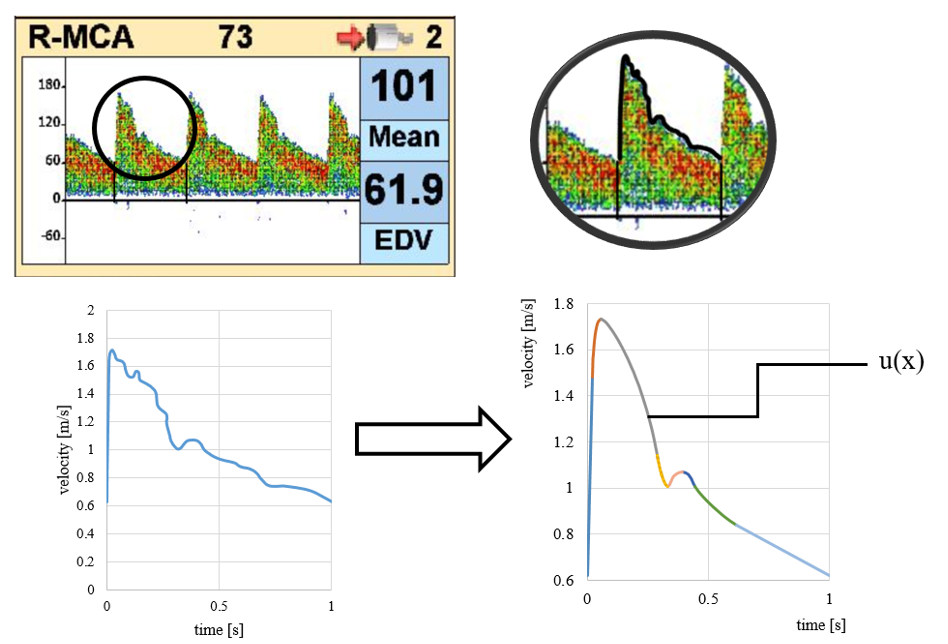
\includegraphics[width=0.7\linewidth]{velocity}}
\caption{Aproksymacja profilu prędkości}
\label{fig:speciation}
\end{figure}


Wszystkie wprowadzane modyfikacje są za każdym razem wdrażane do modelu i zostają przeprowadzane na geometriach tętnic rzeczywistych pacjentów otrzymanych w postaci plików DICOM od  neurochirurgów i chirurgów naczyniowych. Model trójwymiarowy jest uzyskiwany metodą segmentacji tętnicy z programie 3DSlicer oraz wygładzany powierzchniowo w programie ICEM CFD (rys. 3). Tworzenie geometrii tym sposobem jest bardzo czasochłonne, dlatego cały czas trwają poszukiwania lepszej metody obróbki geometrii. Obecnie jest tworzony artykuł, w którym na fragmencie koła Willisa bada się wpływ mniejszych tętniczek na przepływ (co w rozprawie doktorskiej posłuży jako uzasadnienie pominięcia niektórych mniejszych tętnic występujących w rzeczywistych warunkach).

\begin{figure}[H] % Example image
\center{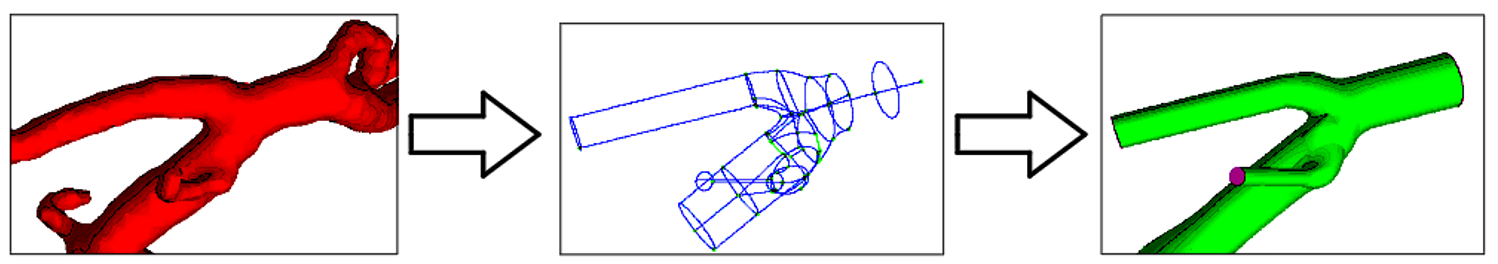
\includegraphics[width=1\linewidth]{geometry}}
\caption{Proces tworzenia geometrii}
\label{fig:speciation}
\end{figure}


Rozpoczęto również prace na stworzeniem modelu bifurkacyjnego tętnicy szyjnej. Obecnie stworzony model geometryczny (w programie Inventor, rys. 4) jest w pełni sparametryzowany: można zmieniać poszczególne wartości średnic tętnic, ich długości oraz kąty rozgałęzienia. Obecnie trwają próby stworzenia siatki strukturalnej dla tego modelu, w celu porównanie wyników obliczeń z siatką niestruktualną (wyniki tego porównania będą opisane w oddzielnym artykule).
\begin{figure}[H] % Example image
\center{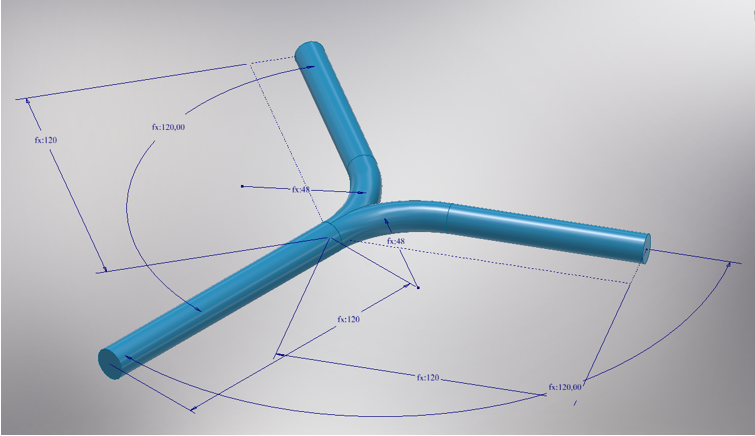
\includegraphics[width=0.65\linewidth]{bifurcation}}
\caption{Geometryczny model rozgałęzienia}
\label{fig:speciation}
\end{figure}


Zadania na przyszły rok obejmują bardziej zaawansowane prace: nad modelem elastycznej ścianki (wymagają one dogłębnych badań w dziedzinie wytrzymałości materiałów) i stworzenie stanowiska do walidacji stosowanych w modelach turbulencji (czasopisma związane stricte z numeryczną mechaniką płynów wymagają walidacji i głównie na ten cel jest tworzone stanowisko). 
Koncepcja stanowiska została już opracowana w programie Fusion 360 (rys. 5). Będzie ona rozwijana w drugiej połowie 2019 roku.
\begin{figure}[H] % Example image
\center{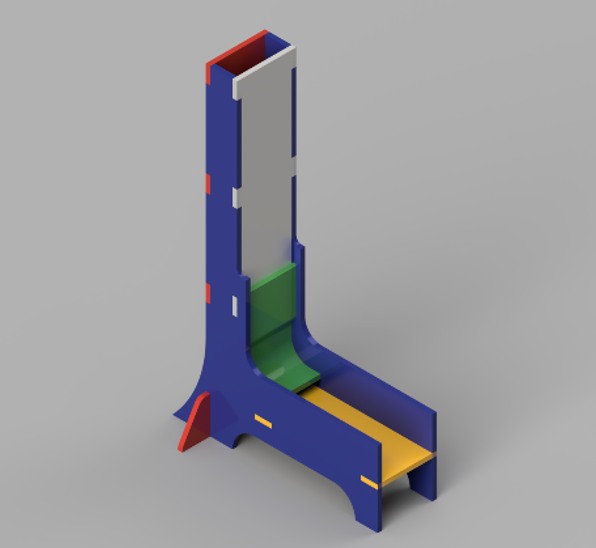
\includegraphics[width=0.65\linewidth]{laboratory}}
\caption{Koncepcja stanowiska laboratoryjnego}
\label{fig:speciation}
\end{figure}
Ostatni rok doktoratu będzie poświęcony na symulacje FSI, tworzenie programu (głównie pod kątem jego optymalizacji i interfejsu, ponieważ części składowe będą już stworzone wcześniej) oraz pisanie rozprawy doktorskiej (jednak na tym etapie założono, że część teoretyczna doktoratu będzie już gotowa). Obrona pracy jest planowana na początek drugiej połowy 2021 roku. Otwarcie przewodu doktorskiego nastąpi we wrześniu 2018 roku. Rozprawa będzie napisana w języku angielskim.


%\begin{wrapfigure}{l}{0.4\textwidth} % Inline image example
%  \begin{center}
%    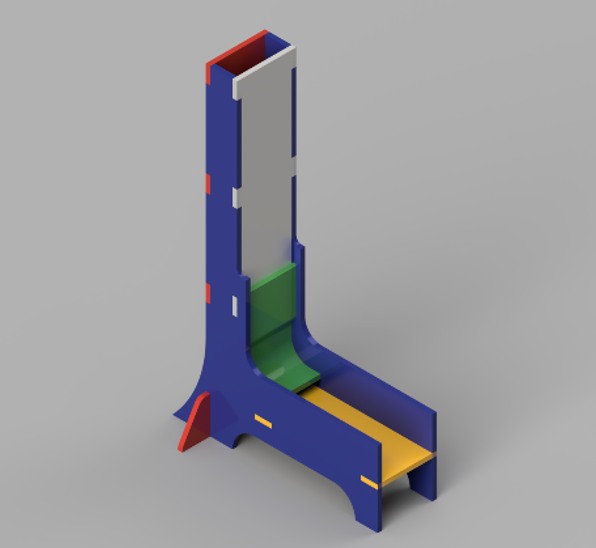
\includegraphics[width=0.38\textwidth]{laboratory}
%  \end{center}
%  \caption{Koncepcja stanowiska laboratoryjnego}
%\end{wrapfigure}



%----------------------------------------------------------------------------------------
%	OKREŚLENIE METOD BADAWCZYCH
%----------------------------------------------------------------------------------------

\section{Określenie metod badawczych}

Badania numeryczne będą prowadzone w środowisku AnsysFluent. Na stan obecny, planuje się przeprowadzenie tych samych symulacji za pomocą oprogramowania OpenFOAM. Ansys Fluent jest oprogramowaniem płatnym, co uniemożliwia rozpowszechnienie modelu na szerszą skalę. Jest jednak bardzo dobrze zoptymalizowany i pozwala uzyskać miarodajne rezultaty bez potrzeby wdrażania skomplikowanych procedur numerycznych. Model ten zostanie później "przeniesiony" do OpenFOAM’a i za pomocą modyfikacji kodu zostanie podjęta próba uzyskania wyników symulacji podobnych do tych, jakie uzyskano za pomocą Fluenta.

%----------------------------------------------------------------------------------------
%	SPODZIEWANE WYNIKI I REZULTATY
%----------------------------------------------------------------------------------------

\section{Spodziewane wyniki i rezultaty}

Stworzony model będzie w możliwie jak największym stopniu odzwierciedlał warunki rzeczywiste. Oczywistym jest, że nie jest realne, by jakikolwiek model w pełni odzwierciedlał rzeczywisty przepływ krwi. Rezultatem pracy ma być uzyskanie modelu, którego stopień dokładności będzie wystarczający dla chirurgów do diagnozy i przewidywania rozwoju schorzeń.


Oprogramowanie będzie mogło być wykorzystywane w trzech (lub czterech) zasadniczych celach:
\begin{itemize}
\item przewidywanie czasu wzrostu złogów do poziomu niebezpiecznego,
\item klasyfikacja pacjentów do grupy ryzyka poprzez genetycznie uwarunkowaną niekorzystną geometrię tętnicy szyjnej,
\item dostosowanie geometrii łatki operacyjnej wszywanej w miejsce rozcięcia tętnicy.
\end{itemize}

Czwartym zastosowaniem modelu byłaby możliwość przewidywania wzrostu i ewentualnego pęknięcia tętniaka. Jednak na tym etapie prac nie jest pewne, czy badania daną spodziewany efekt i czy nie będzie wymagane wdrożenie dodatkowych zagadnień i parametrów. Dlatego nie jest to obecnie zaliczane do „pewnych” wyników uzyskanych w rozprawie doktorskiej. Jeśli model nie będzie spełniał wymagań odnoście symulowania wzrostu tętniaków, w rozprawie zostaną opisane dotychczas uzyskane rezultaty i plan rozwoju tych badań w przyszłości.


Istotną zaletą stworzonego modelu będzie jego dostępność. Będzie on rozpowszechniony w postaci oprogramowania opensource’owego, z którego każdy będzie mógł korzystać, ulepszać i modyfikować wg własnych potrzeb. Zostanie również on przetestowany przez nie tylko chirurgów, z którymi została nawiązana współpraca, ale też ludzi zajmujących się biomechaniką przepływów. 
Planuje się również rozszerzenie modelu (po doktoracie) do innych zagadnień związanych z chirurgią naczyniową:
\begin{itemize}
\item wprowadzenie parametrów pozwalających na sumulację przepływu w tętnicy udowej,
\item implementacja stentów w tętnicy i badania zaburzeń przepływu pod wpływem ich wprowadzenia,
\item symulacja wzrostu tętniaków w tętnicy udowej i ich ewentualnych nieszczelności poprzez zjawisko przesączania,
\item wprowadzenie możliwości „sztucznego” osłabiania ścianki w miejscach, w których często dochodzi do tworzenia tętniaków.
\end{itemize}




%----------------------------------------------------------------------------------------
%	MAJOR SECTION X - TEMPLATE - UNCOMMENT AND FILL IN
%----------------------------------------------------------------------------------------

%\section{Content Section}

%\subsection{Subsection 1} % Sub-section

% Content

%------------------------------------------------

%\subsection{Subsection 2} % Sub-section

% Content

%----------------------------------------------------------------------------------------
%	CONCLUSION
%----------------------------------------------------------------------------------------



%----------------------------------------------------------------------------------------
%	BIBLIOGRAPHY
%----------------------------------------------------------------------------------------
%
%\begin{thebibliography}{99} % Bibliography - this is intentionally simple in this template
%
%\bibitem[Figueredo and Wolf, 2009]{Figueredo:2009dg}
%Figueredo, A.~J. and Wolf, P. S.~A. (2009).
%\newblock Assortative pairing and life history strategy - a cross-cultural
%  study.
%\newblock {\em Human Nature}, 20:317--330.
% 
%\end{thebibliography}

%----------------------------------------------------------------------------------------

\end{document}